\newpage
\section{Monolayers}
\label{sec:mono}

\subsection{Methods}

The following is conducted for two different unknown TMDCs:
Firstly the scotch tape technique is used, to separate the layers from a thick crystal and then into thinner pieces, until monolayers are likely to exist on the tape.
These layers are then transferred to a gel strip, from which they are subsequently transferred onto a silicon wafer that has an \SI{80}{nm} thick SiO$_2$ layer on top.

In order to now find pieces on the wafer that are monolayers, a common optical microscope is used, utilizing the fact that, due to the different refractive indices of Si, the SiO$_2$ and the deposited material, different thicknesses appear in different colors \cite{benameur2011}.
The samples are then transferred to a widefield microscope, a schematic of which is shown in \cref{fig_widefield}.
Its basic principle is to illuminate the sample with a \SI{532}{nm} laser (green lines) to create excitons and measure the photoluminescence light (red lines) in the spectrometer.
Using the white light source allows illuminatation of the sample in order to navigate on it.
The laser line filter is added to sharpen the spectrum emitted from the laser and the longpass filter (cutoff at \SI{560}{nm}) filters the laser's reflection from the photoluminescence spectrum.
The objective lense used is a Nikon 50x and has a numerical aperture of \SI{0.6}{}.
Apart from also having imaging properties, a slit can be inserted into the widefield microscope, to record a spectrum using a basic light spectrometer.
Due to the insertion of the slit, imaging properties in one direction are lost in the process.
For both microscopes (the common optical microscope and the widefield microscope) a sample with a grid of known grid size is used, to get the scale for the images taken of the samples.
For one material two specimen (pieces including monolayers) are examined and for the other one only one specimen is examined.

\begin{figure}[!ht]
    \centering
    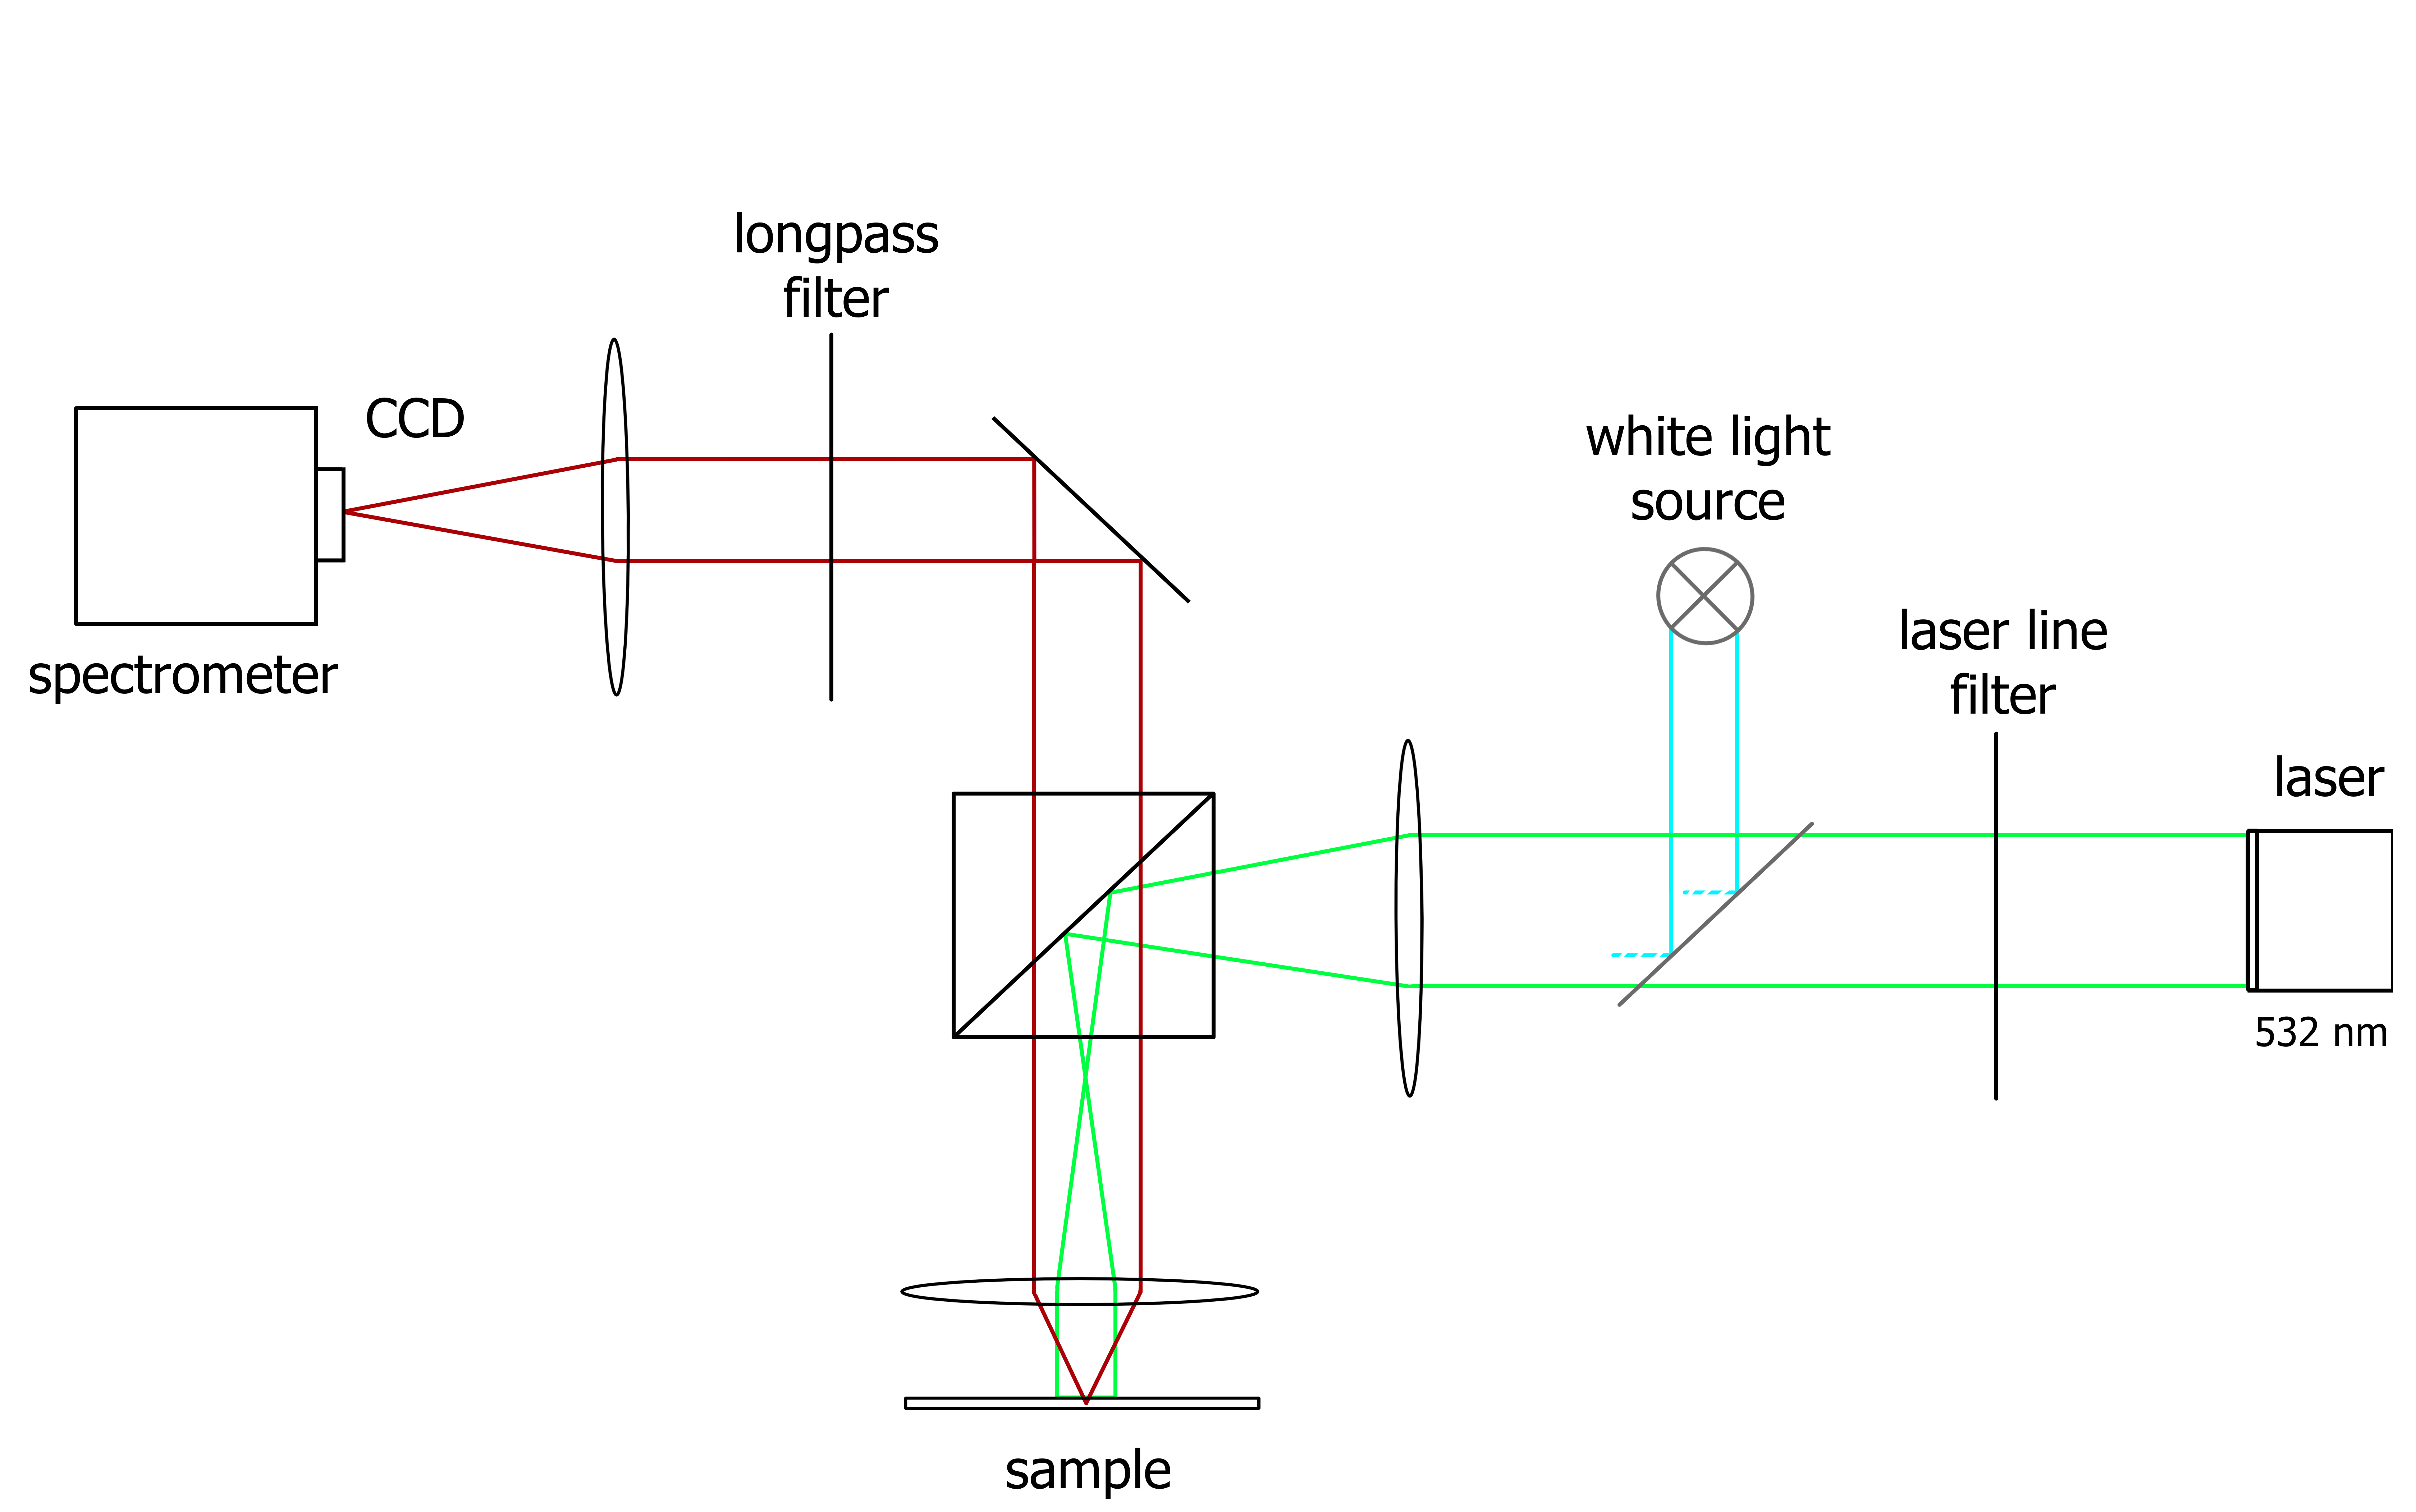
\includegraphics[width=0.8\textwidth]{img/setup1.png}
    \caption{Schematic of the widefield microscope used to record photoluminescence spectra. The detector corresponds to a spectrometer.}
    \label{fig_widefield}
\end{figure}


\subsection{Analysis}

In \crefrange{fig_mono_spec1}{fig_mono_spec3} the images recorded based on substrate interference and the widefield microscope are shown.
As an example, for the first specimen the image containing the spectrum is shown in \cref{fig_mono_spec1_spec}.
In the interference based microscope monolayers appear as fawn (hex color code \#A97E5C), while in the widefield microscope they appear bright white.
From these images for each specimen the spectrum is calculated by summing over multiple lines of pixels and can be seen in \cref{fig_mono_1dspectra}.

\begin{figure}[H]
    \centering
    \begin{subfigure}{0.3\textwidth}
        \centering
        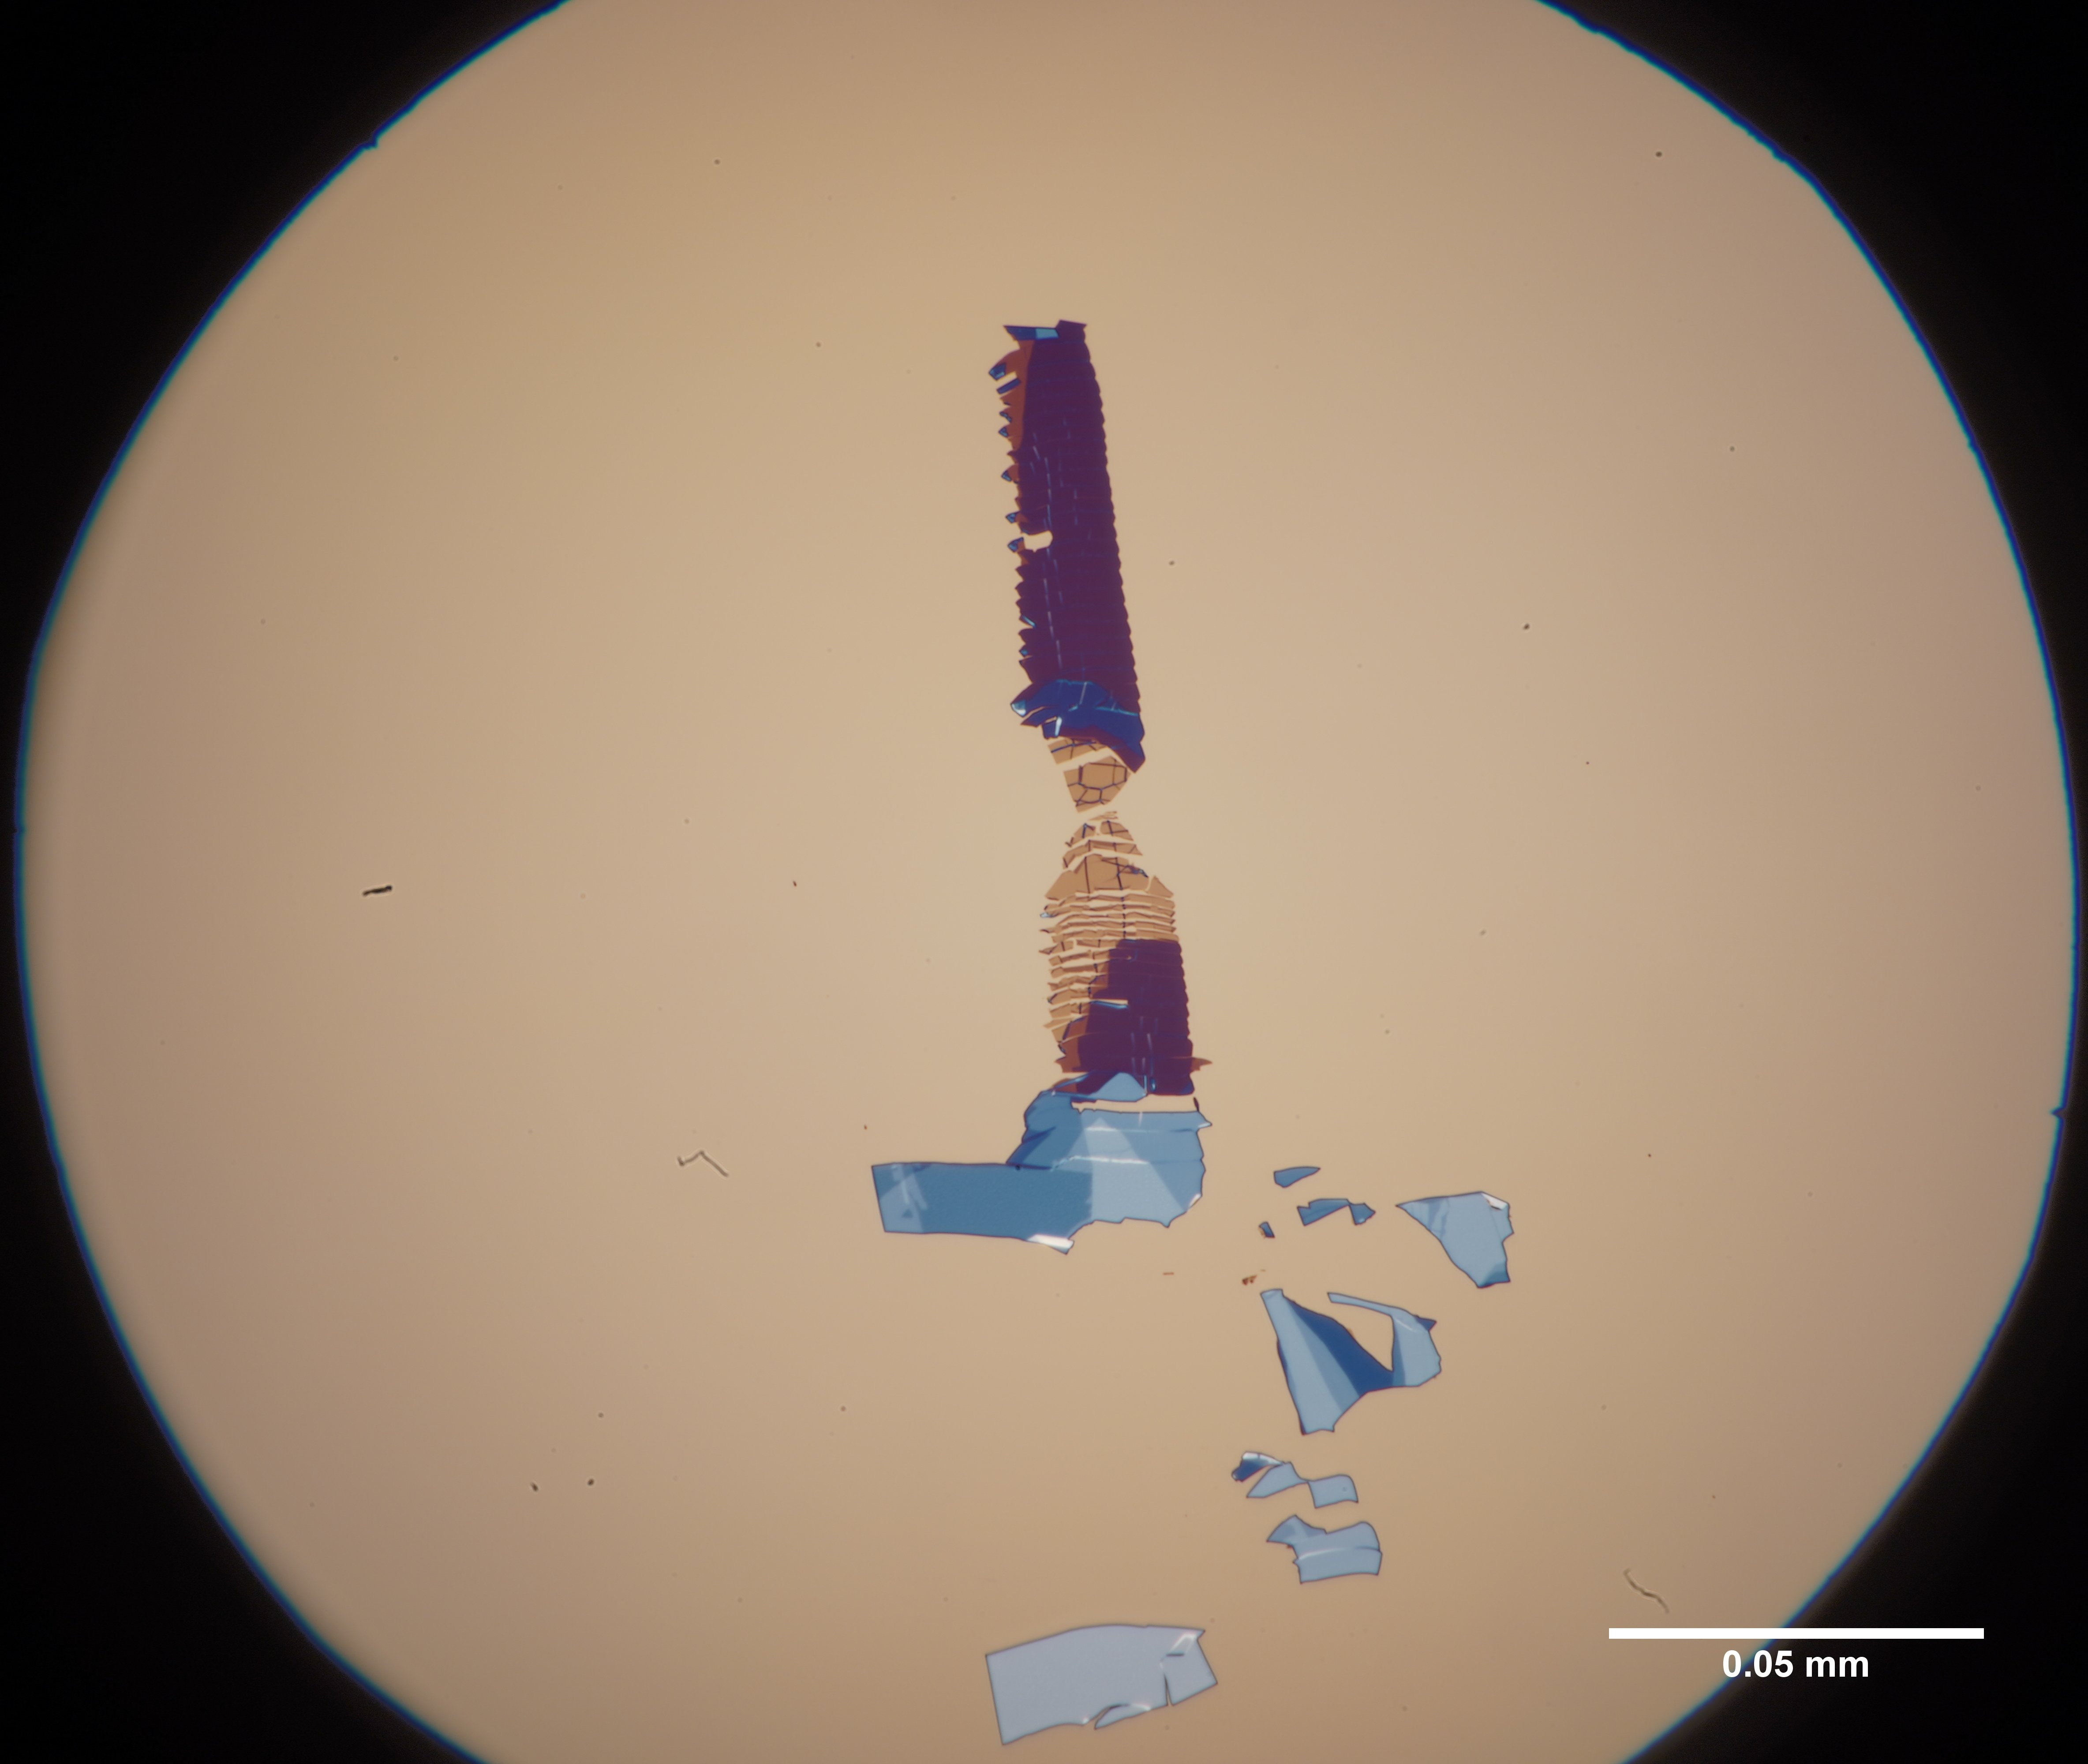
\includegraphics[width=1.0\textwidth]{img/output_t1/M1_3_100_adj}
        \caption{interference}
	      \label{fig_mono_spec1_int}
    \end{subfigure}
    %\hfill
    \begin{subfigure}{0.24\textwidth}
        \centering
        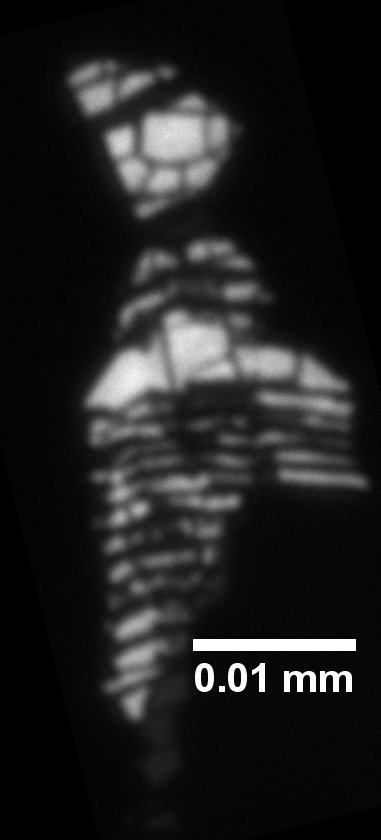
\includegraphics[width=\textwidth]{img/output_t1/M1_3_50_adj_photo}
        \caption{widefield}
	      \label{fig_mono_spec1_wide}
    \end{subfigure}
    \begin{subfigure}{0.75\textwidth}
        \centering
        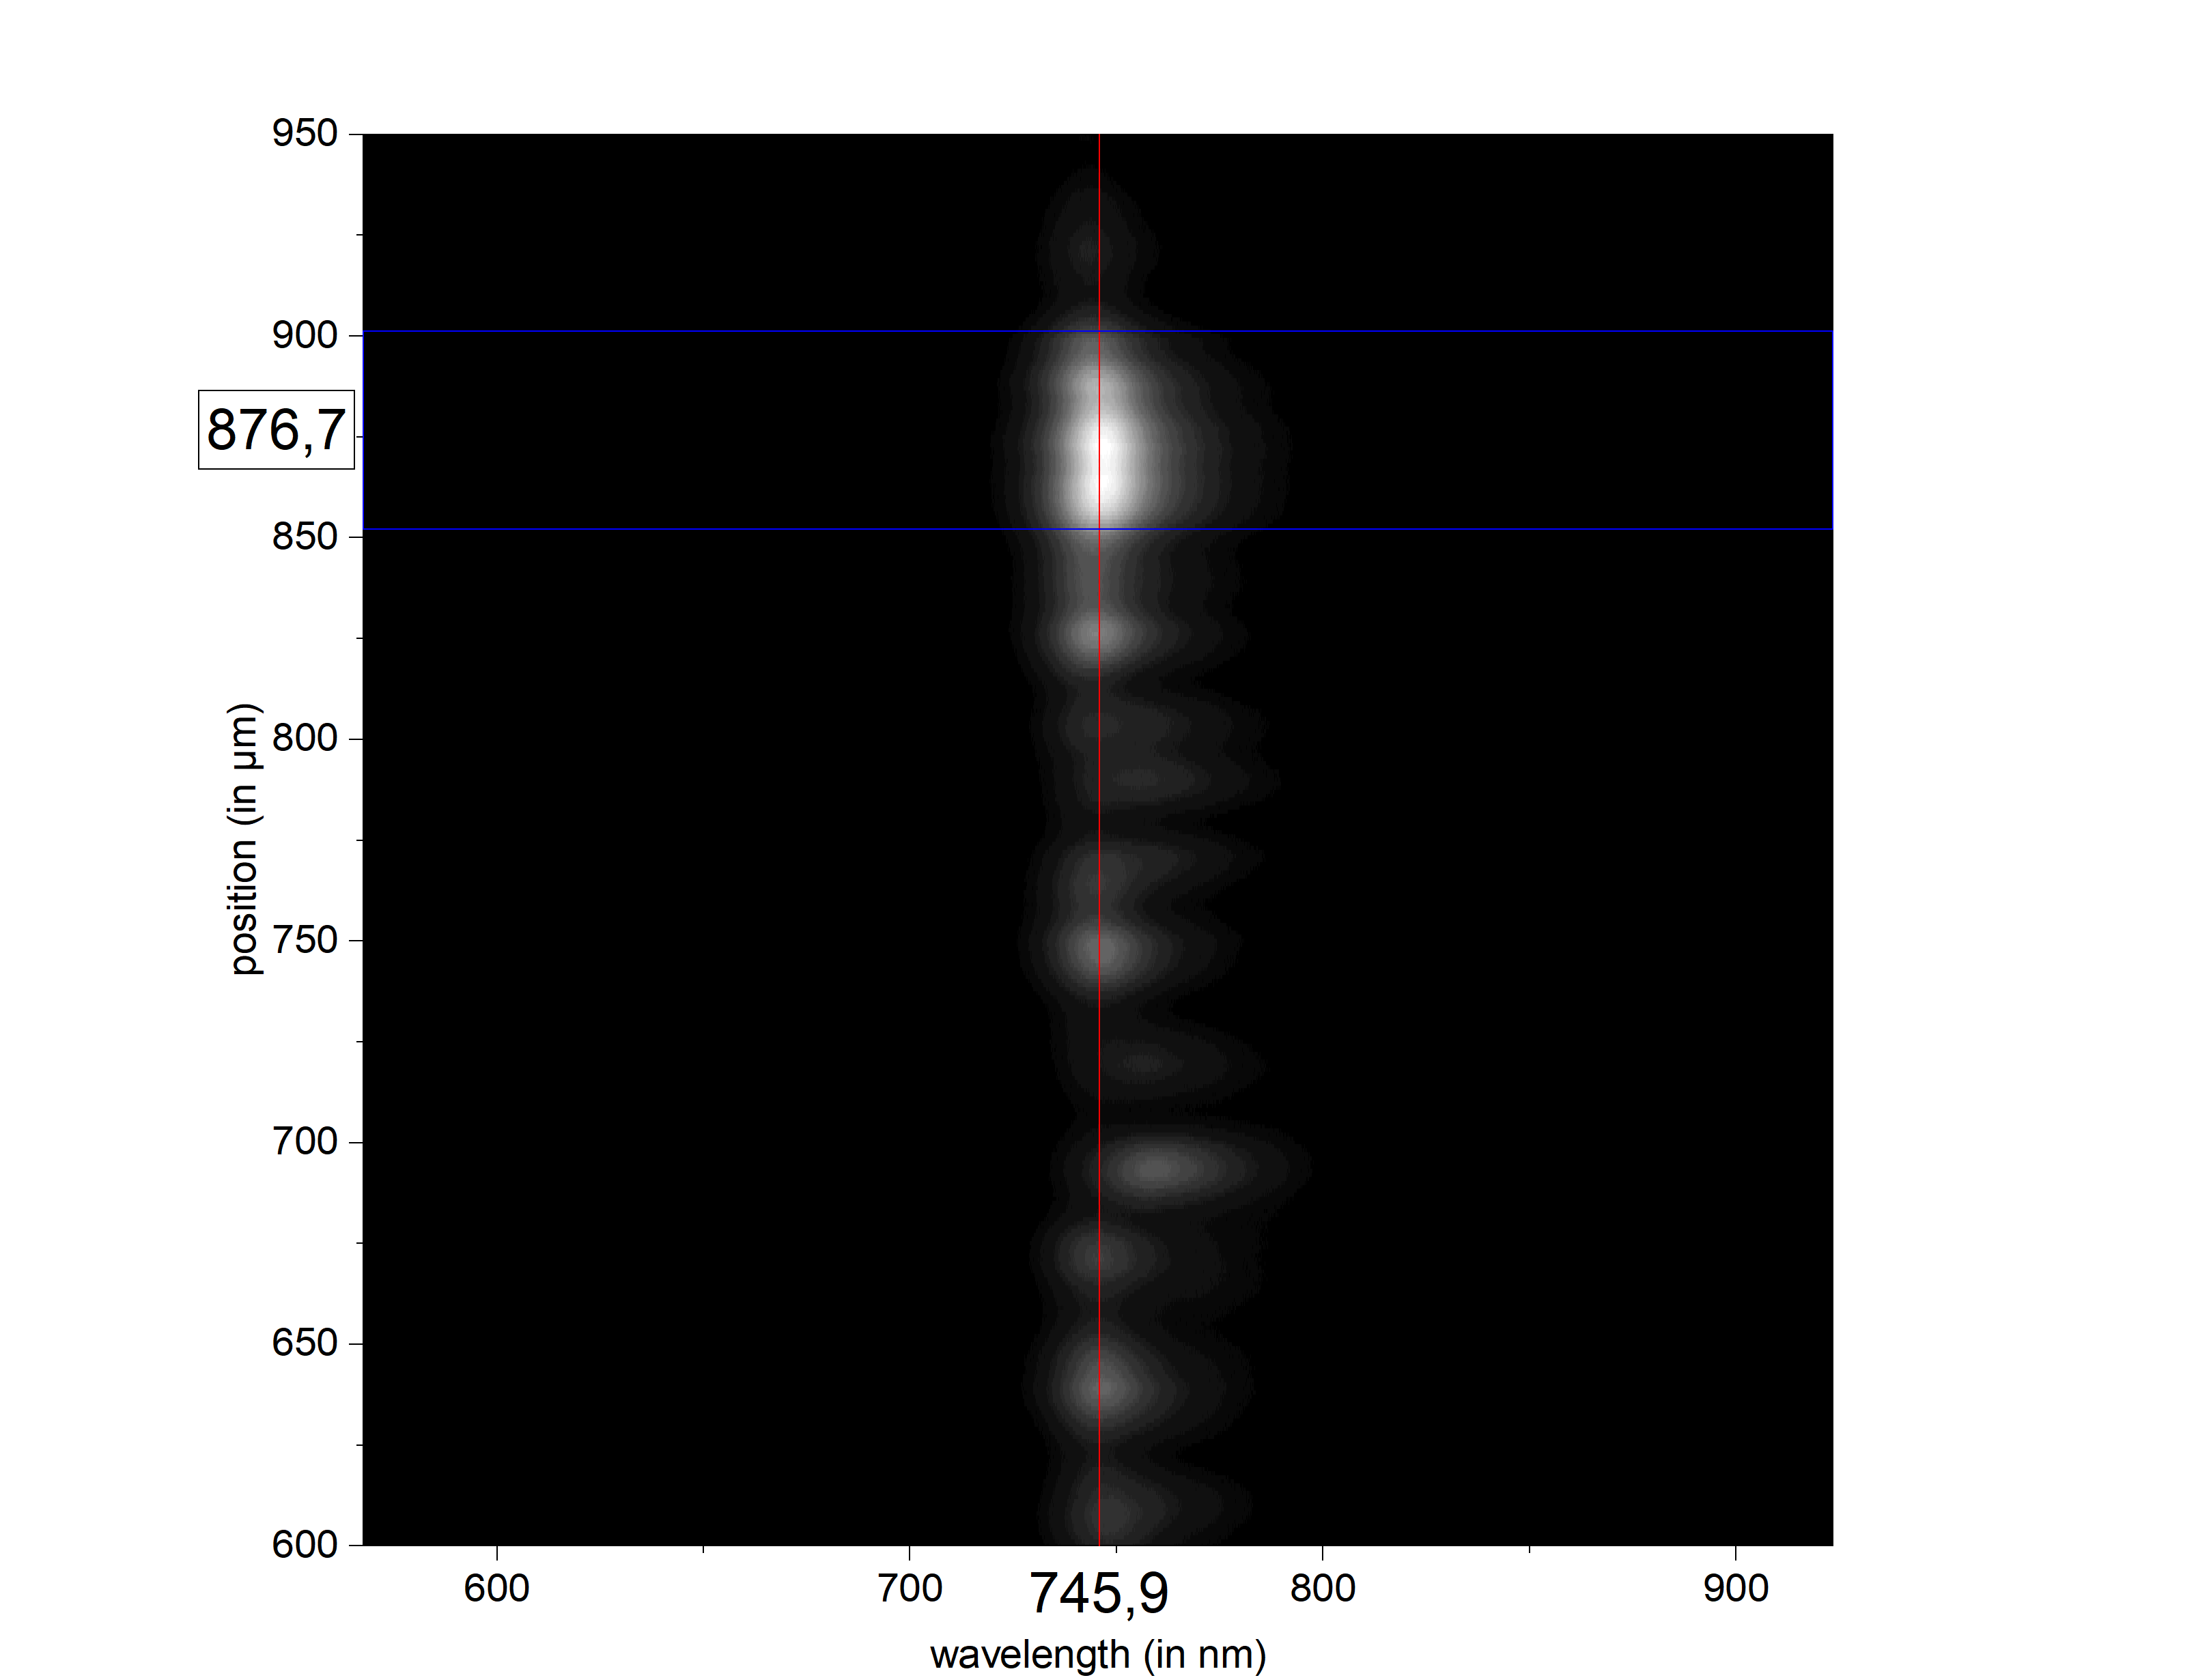
\includegraphics[width=\textwidth]{img/output_t1/bild_m1-3}
        \caption{spectrum}
	      \label{fig_mono_spec1_spec}
    \end{subfigure}
    \caption{Optical microscopy images for specimen 1 of material 1 obtained by the interference based microscope and the widefield microscope. Additionally the image containing the spectrum in one direction is shown and the part that is used for the spectrum in \cref{fig_mono_1dspectra} lies between the blue lines.}
	\label{fig_mono_spec1} % 3->1
\end{figure}

\begin{figure}[H]
    \centering
    \begin{subfigure}{0.4\textwidth}
        \centering
        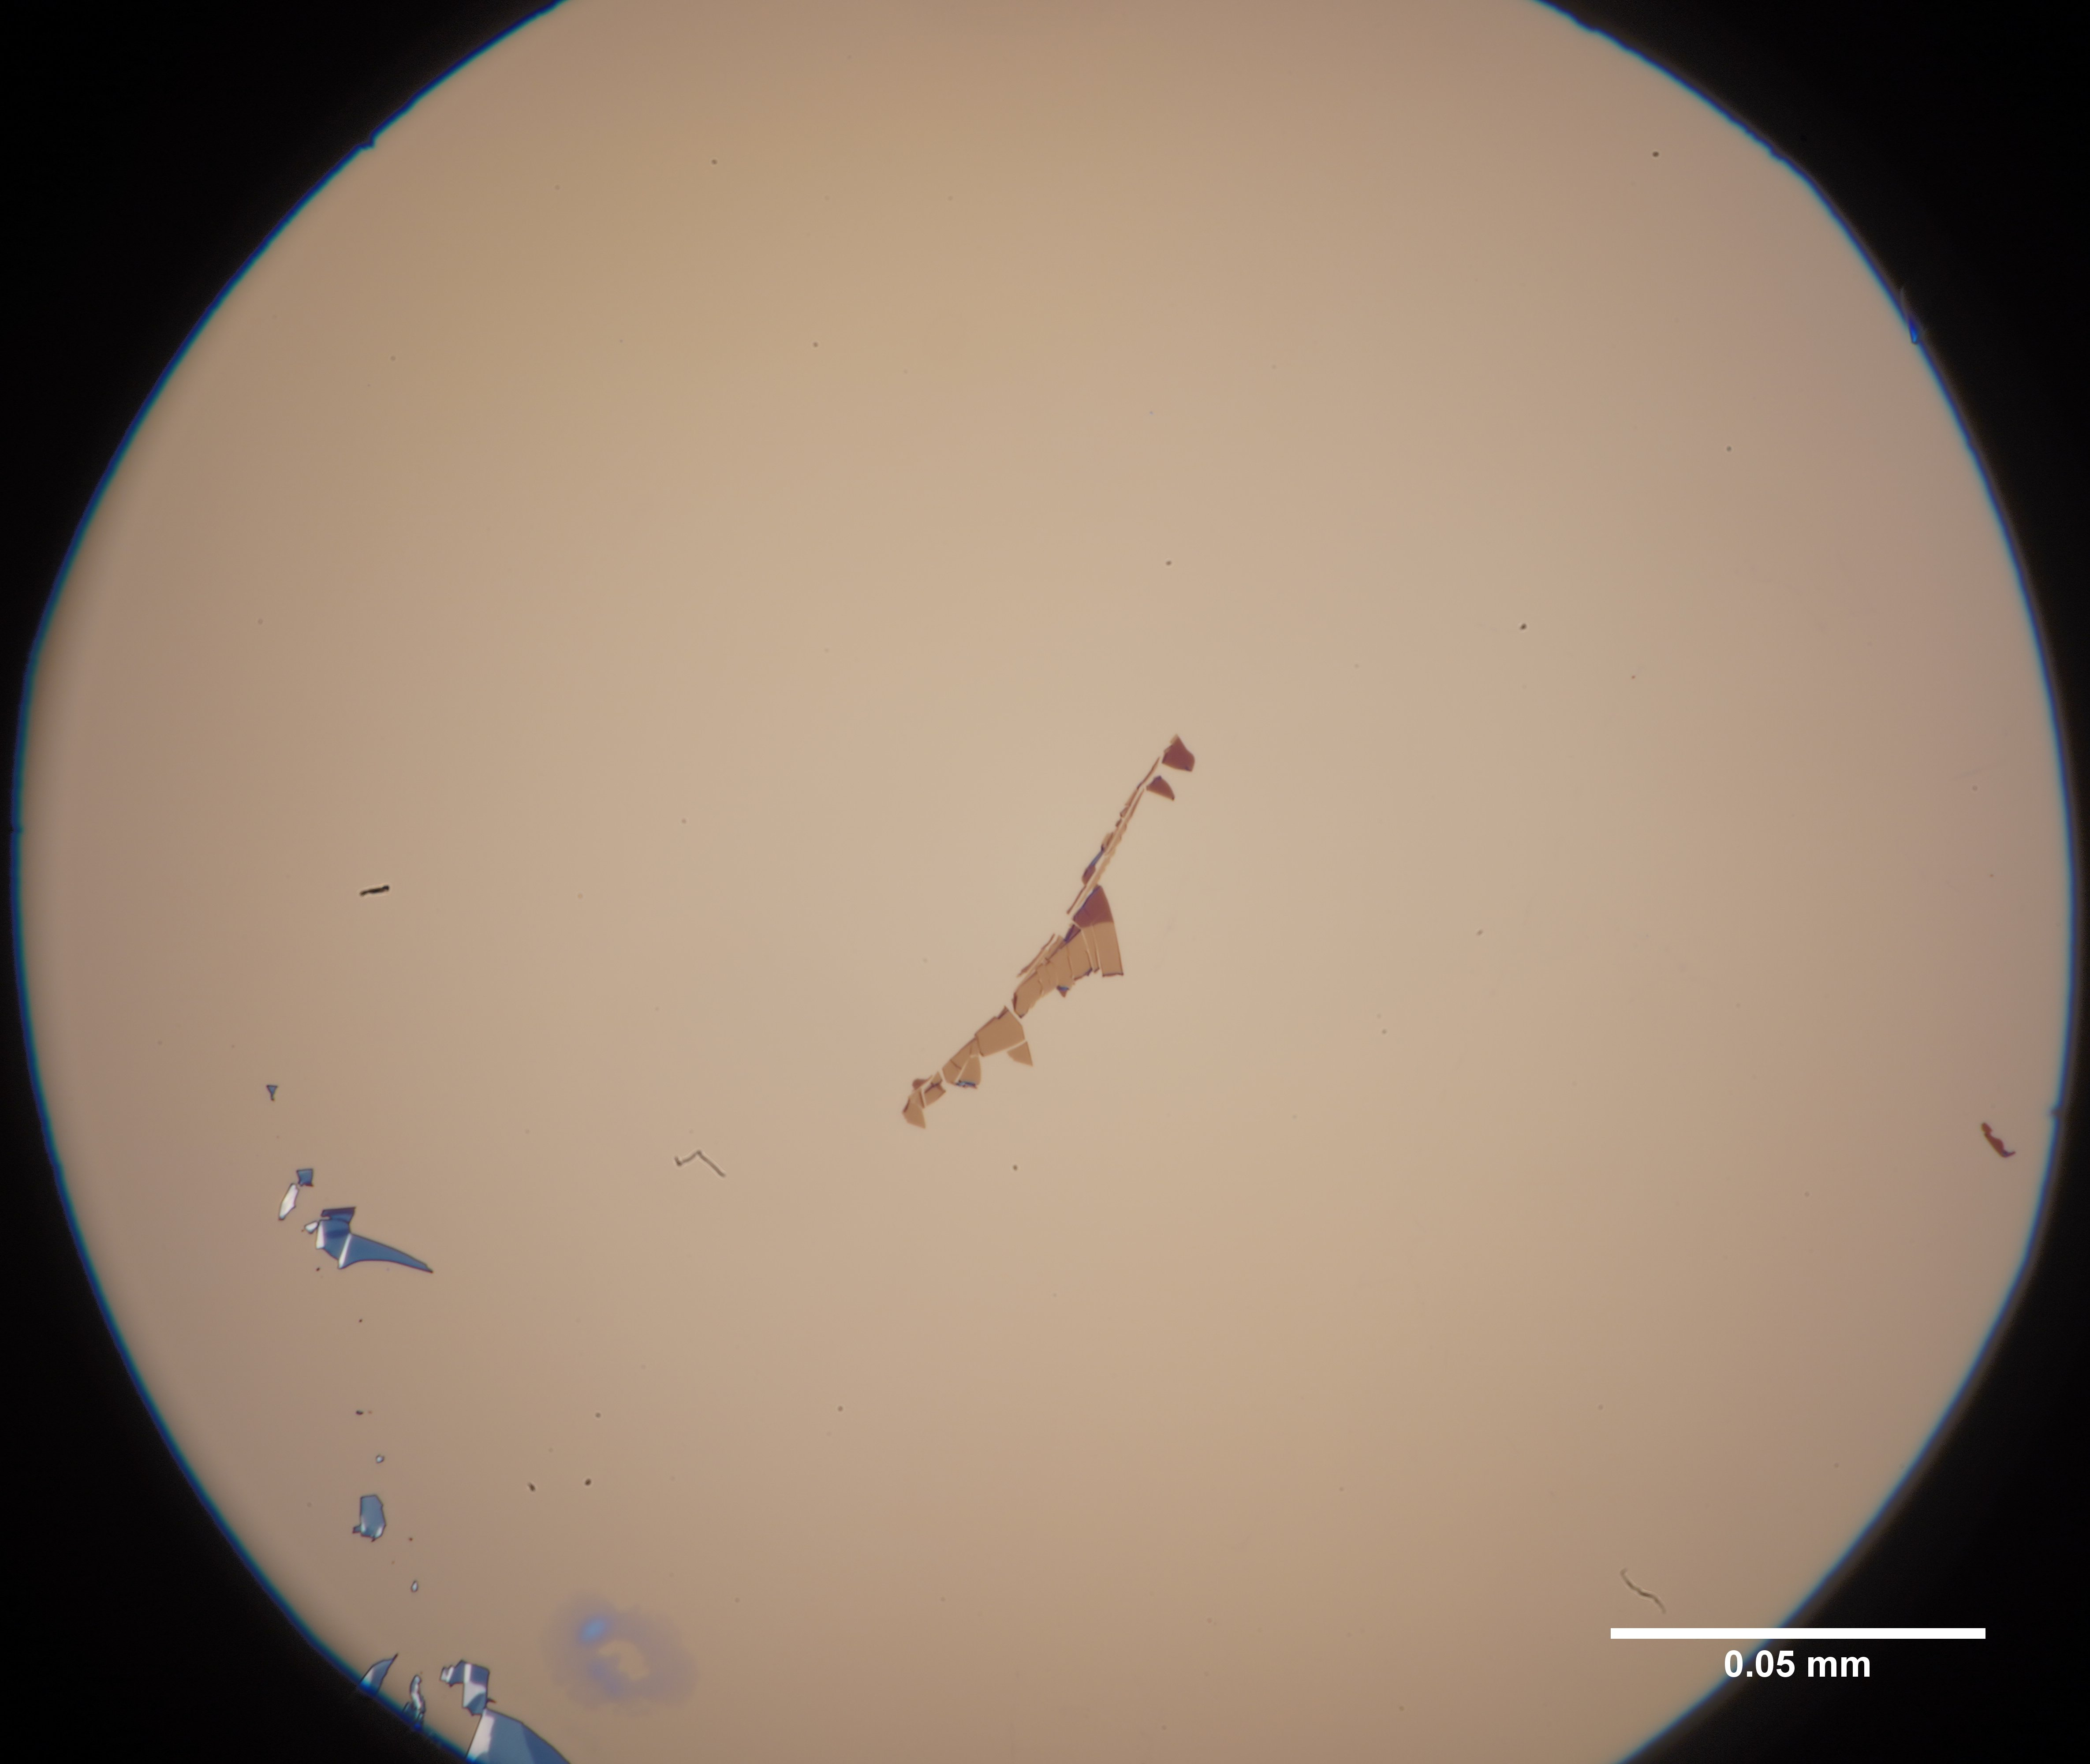
\includegraphics[width=\textwidth]{img/output_t1/M1_2_100_adj}
        \caption{interference}
	      \label{fig_mono_spec2_int}
    \end{subfigure}
    \begin{subfigure}{0.4\textwidth}
        \centering
        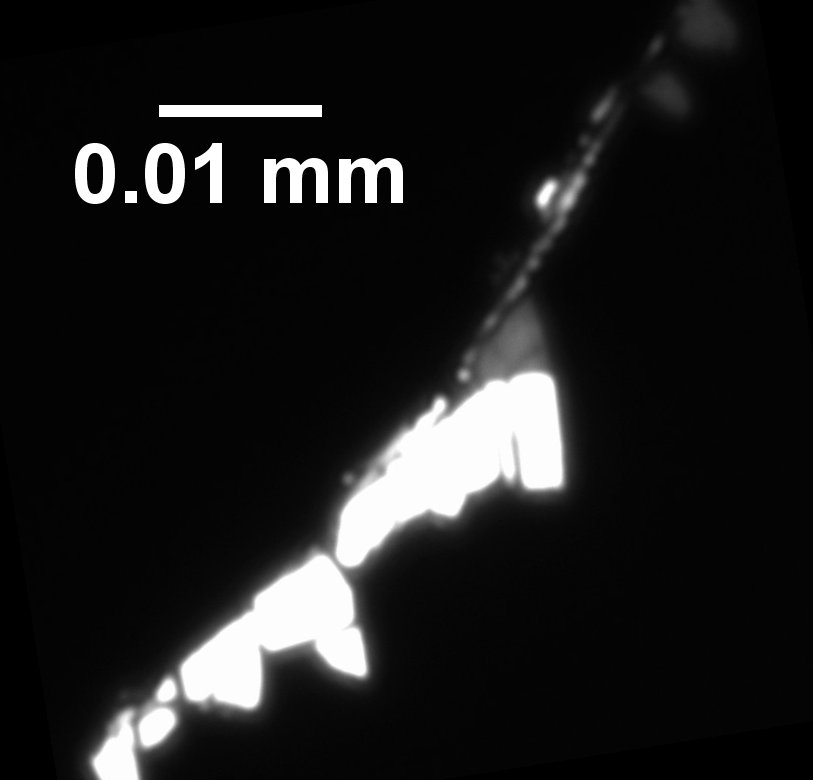
\includegraphics[width=\textwidth]{img/output_t1/M1_2_50_adj_photo}
        \caption{widefield}
	      \label{fig_mono_spec2_wide}
    \end{subfigure}
    \caption{Optical microscopy images for specimen 2 of material 1 obtained by the interference based microscope and the widefield microscope. The region of the monolayer is overexposed so that the thicker parts are also visible.}
	\label{fig_mono_spec2} %2->2
\end{figure}

\begin{figure}[H]
    \centering
    \begin{subfigure}{0.4\textwidth}
        \centering
        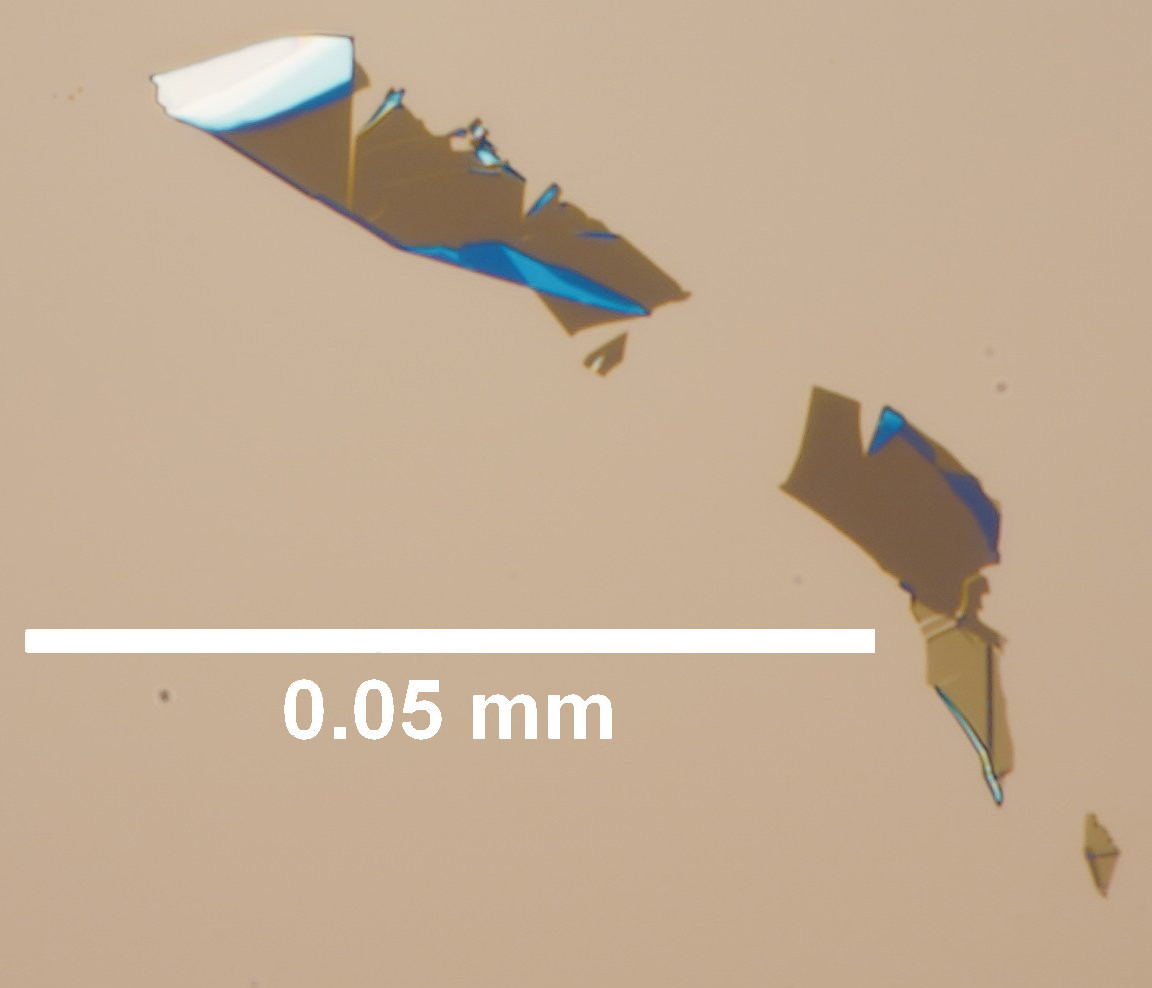
\includegraphics[width=1.0\textwidth]{img/output_t1/M2_1_100_adj}
        \caption{interference}
	      \label{fig_mono_spec3_int}
    \end{subfigure}
    \begin{subfigure}{0.49\textwidth}
        \centering
        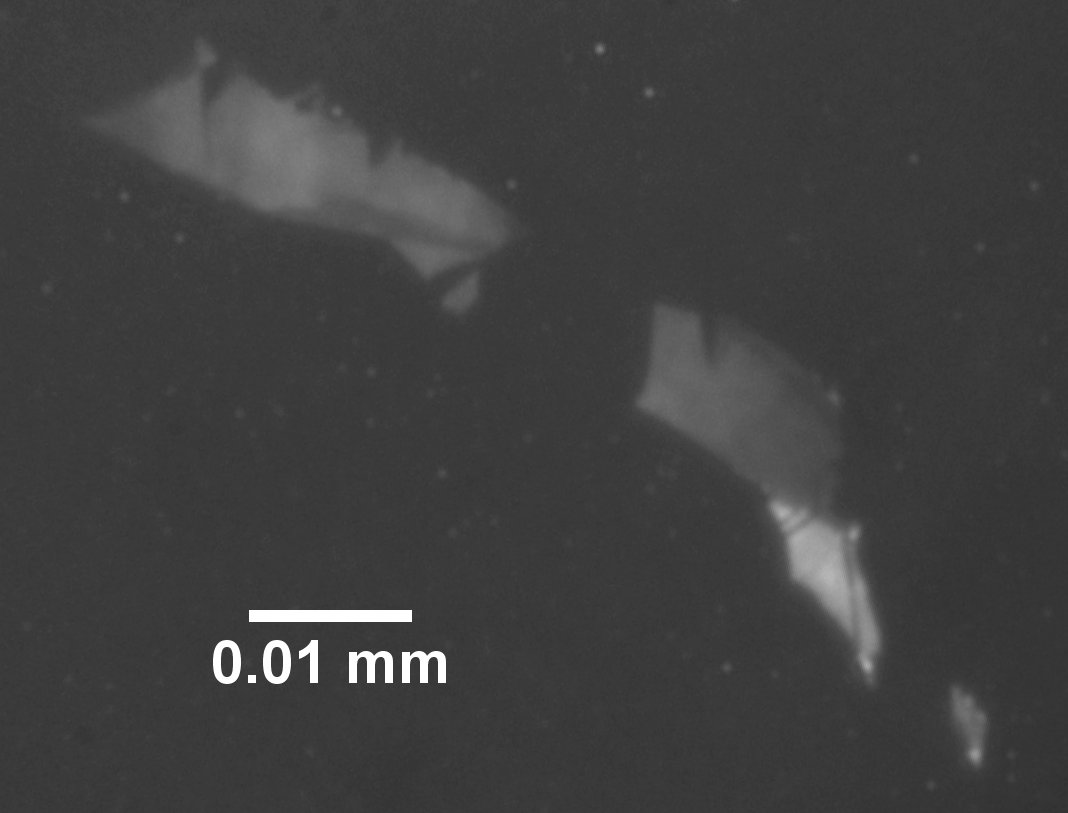
\includegraphics[width=\textwidth]{img/output_t1/M2_1_50_adj_photo4}
        \caption{widefield}
	      \label{fig_mono_spec3_wide}
    \end{subfigure}
    \caption{Optical microscopy images for material 2 obtained by the interference based microscope and the widefield microscope.}
	\label{fig_mono_spec3} %mat2 -> 3
\end{figure}

\begin{figure}[H]
    \centering
    \begin{subfigure}{0.47\textwidth}
        \centering
        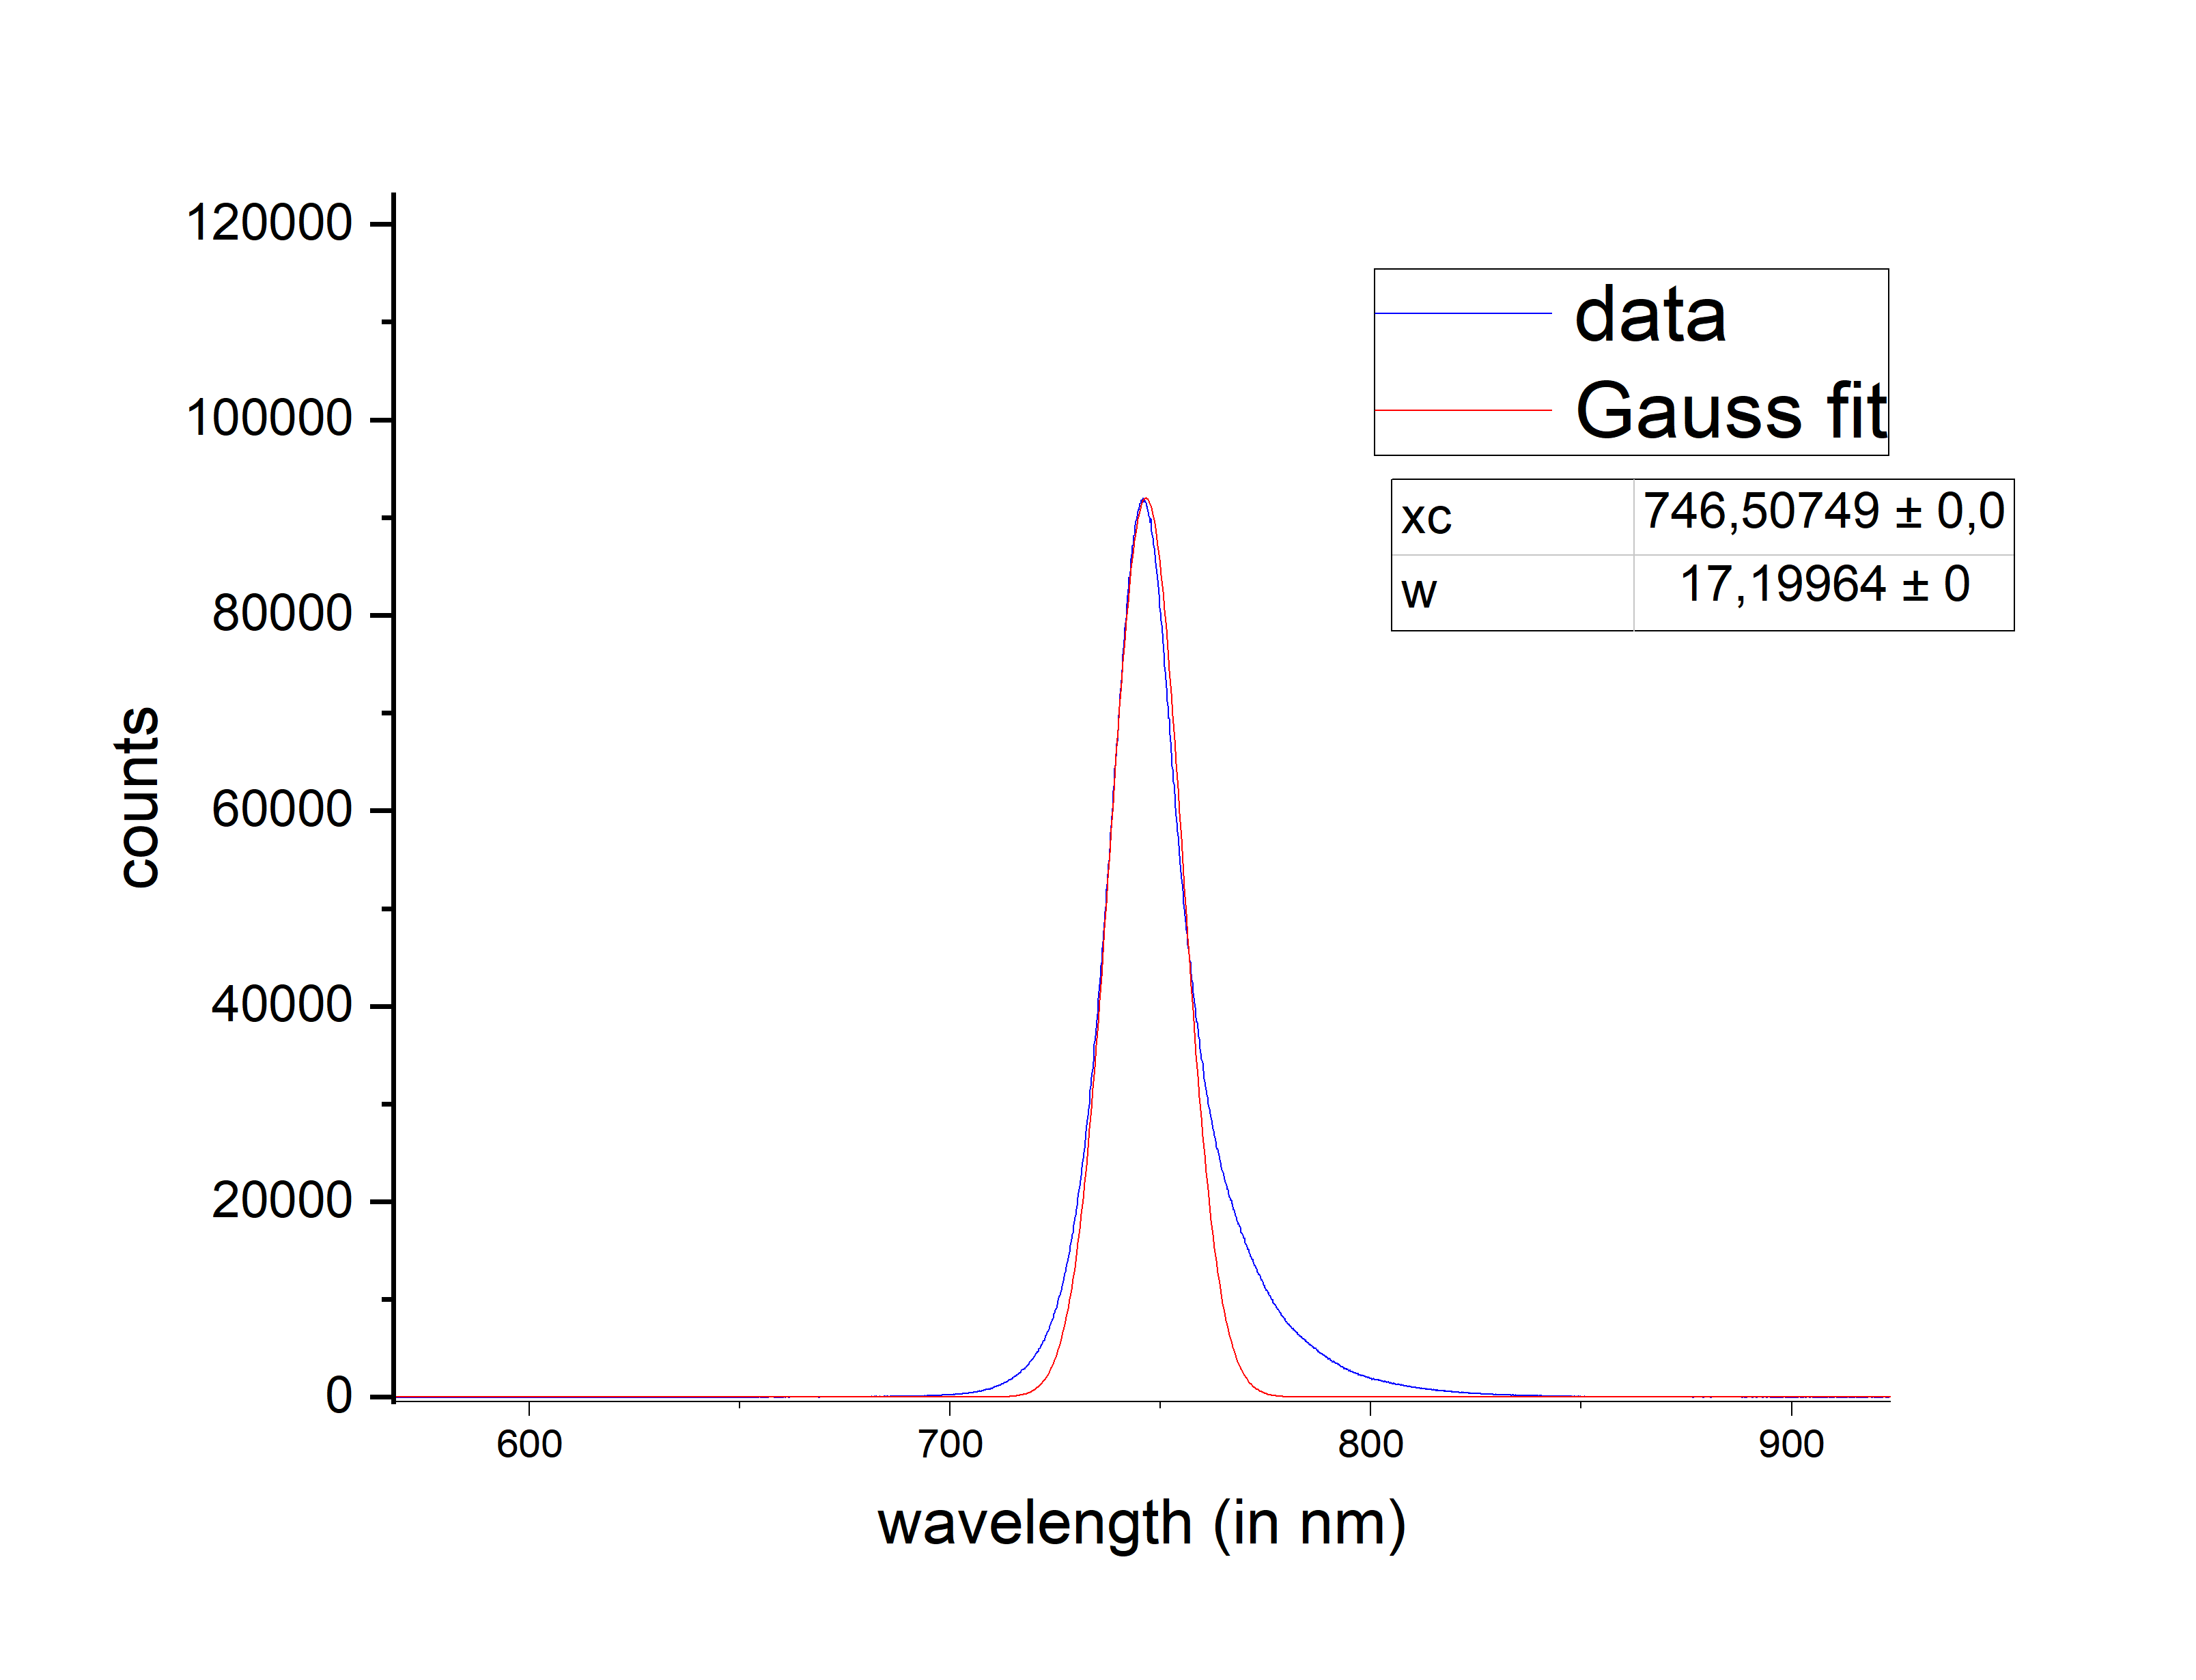
\includegraphics[width=\textwidth]{img/output_t1/spekt_m1-3}
        \caption{mat. 1, spec. 1}
	      \label{fig_mono_spec1_1dspec}
    \end{subfigure}
    \begin{subfigure}{0.47\textwidth}
        \centering
        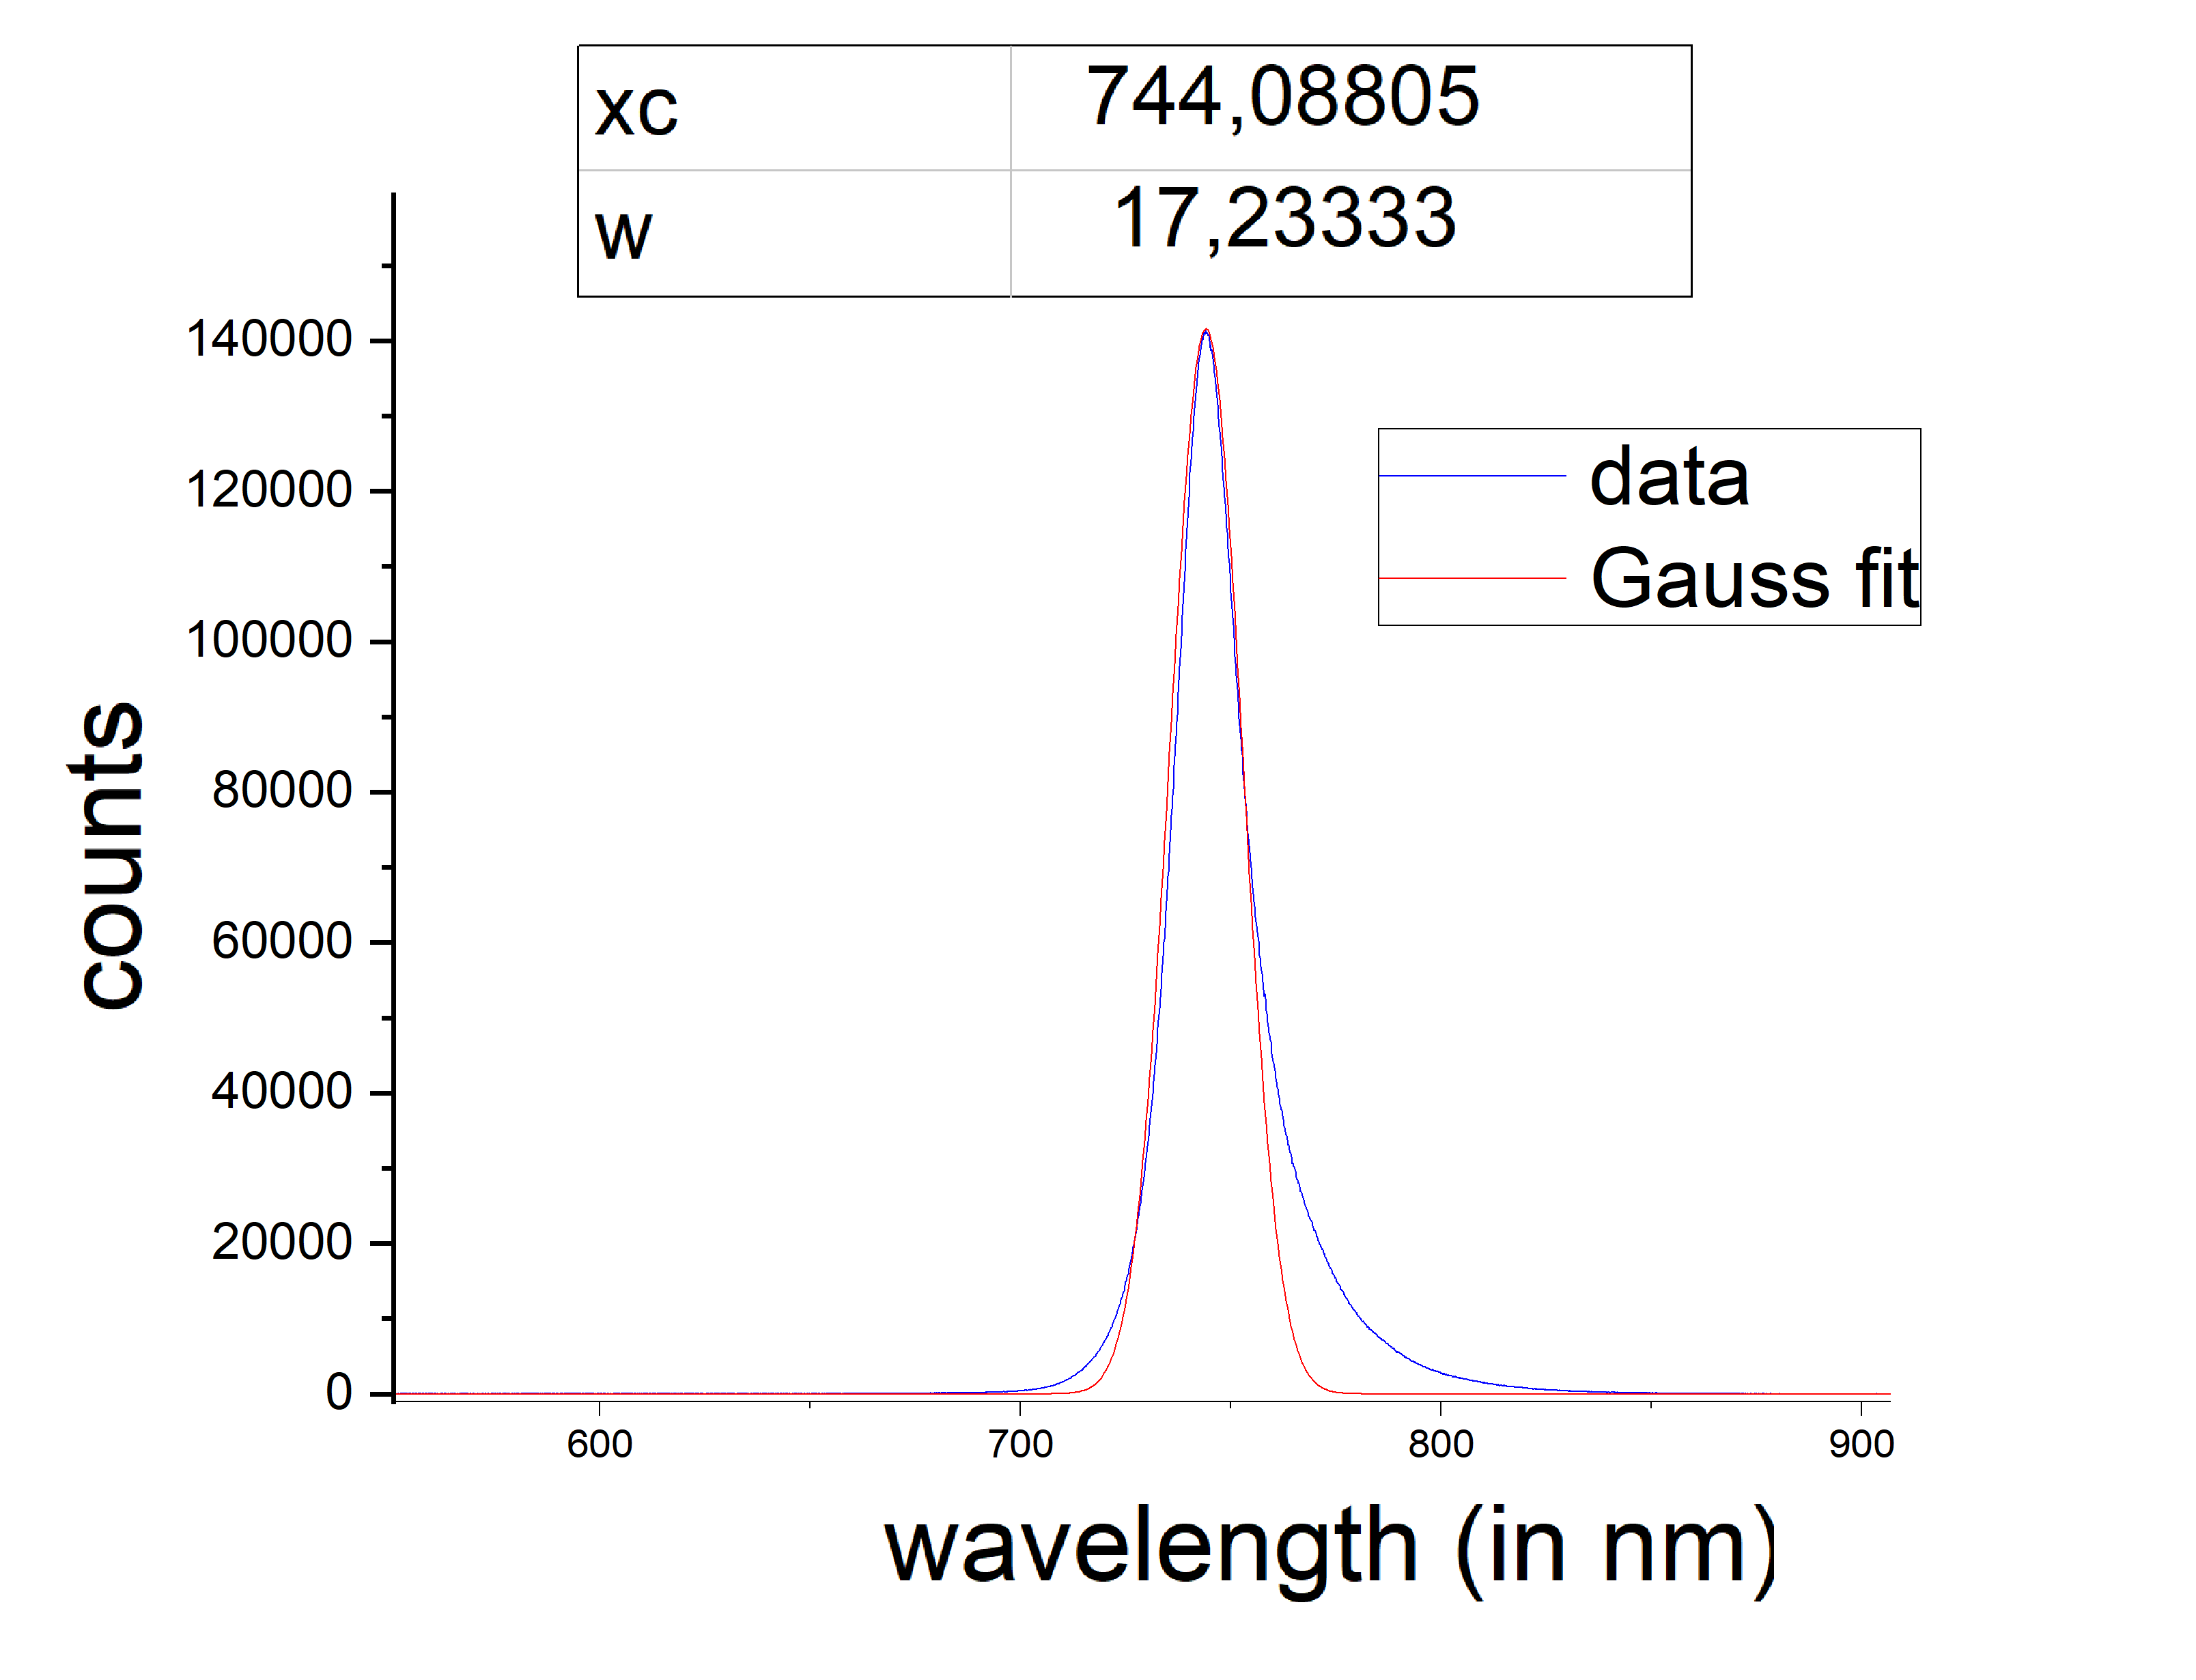
\includegraphics[width=\textwidth]{img/output_t1/spekt_m1-2-1}
        \caption{mat.1, spec. 2}
	      \label{fig_mono_spec2_1dspec}
    \end{subfigure}
    \begin{subfigure}{0.6\textwidth}
        \centering
        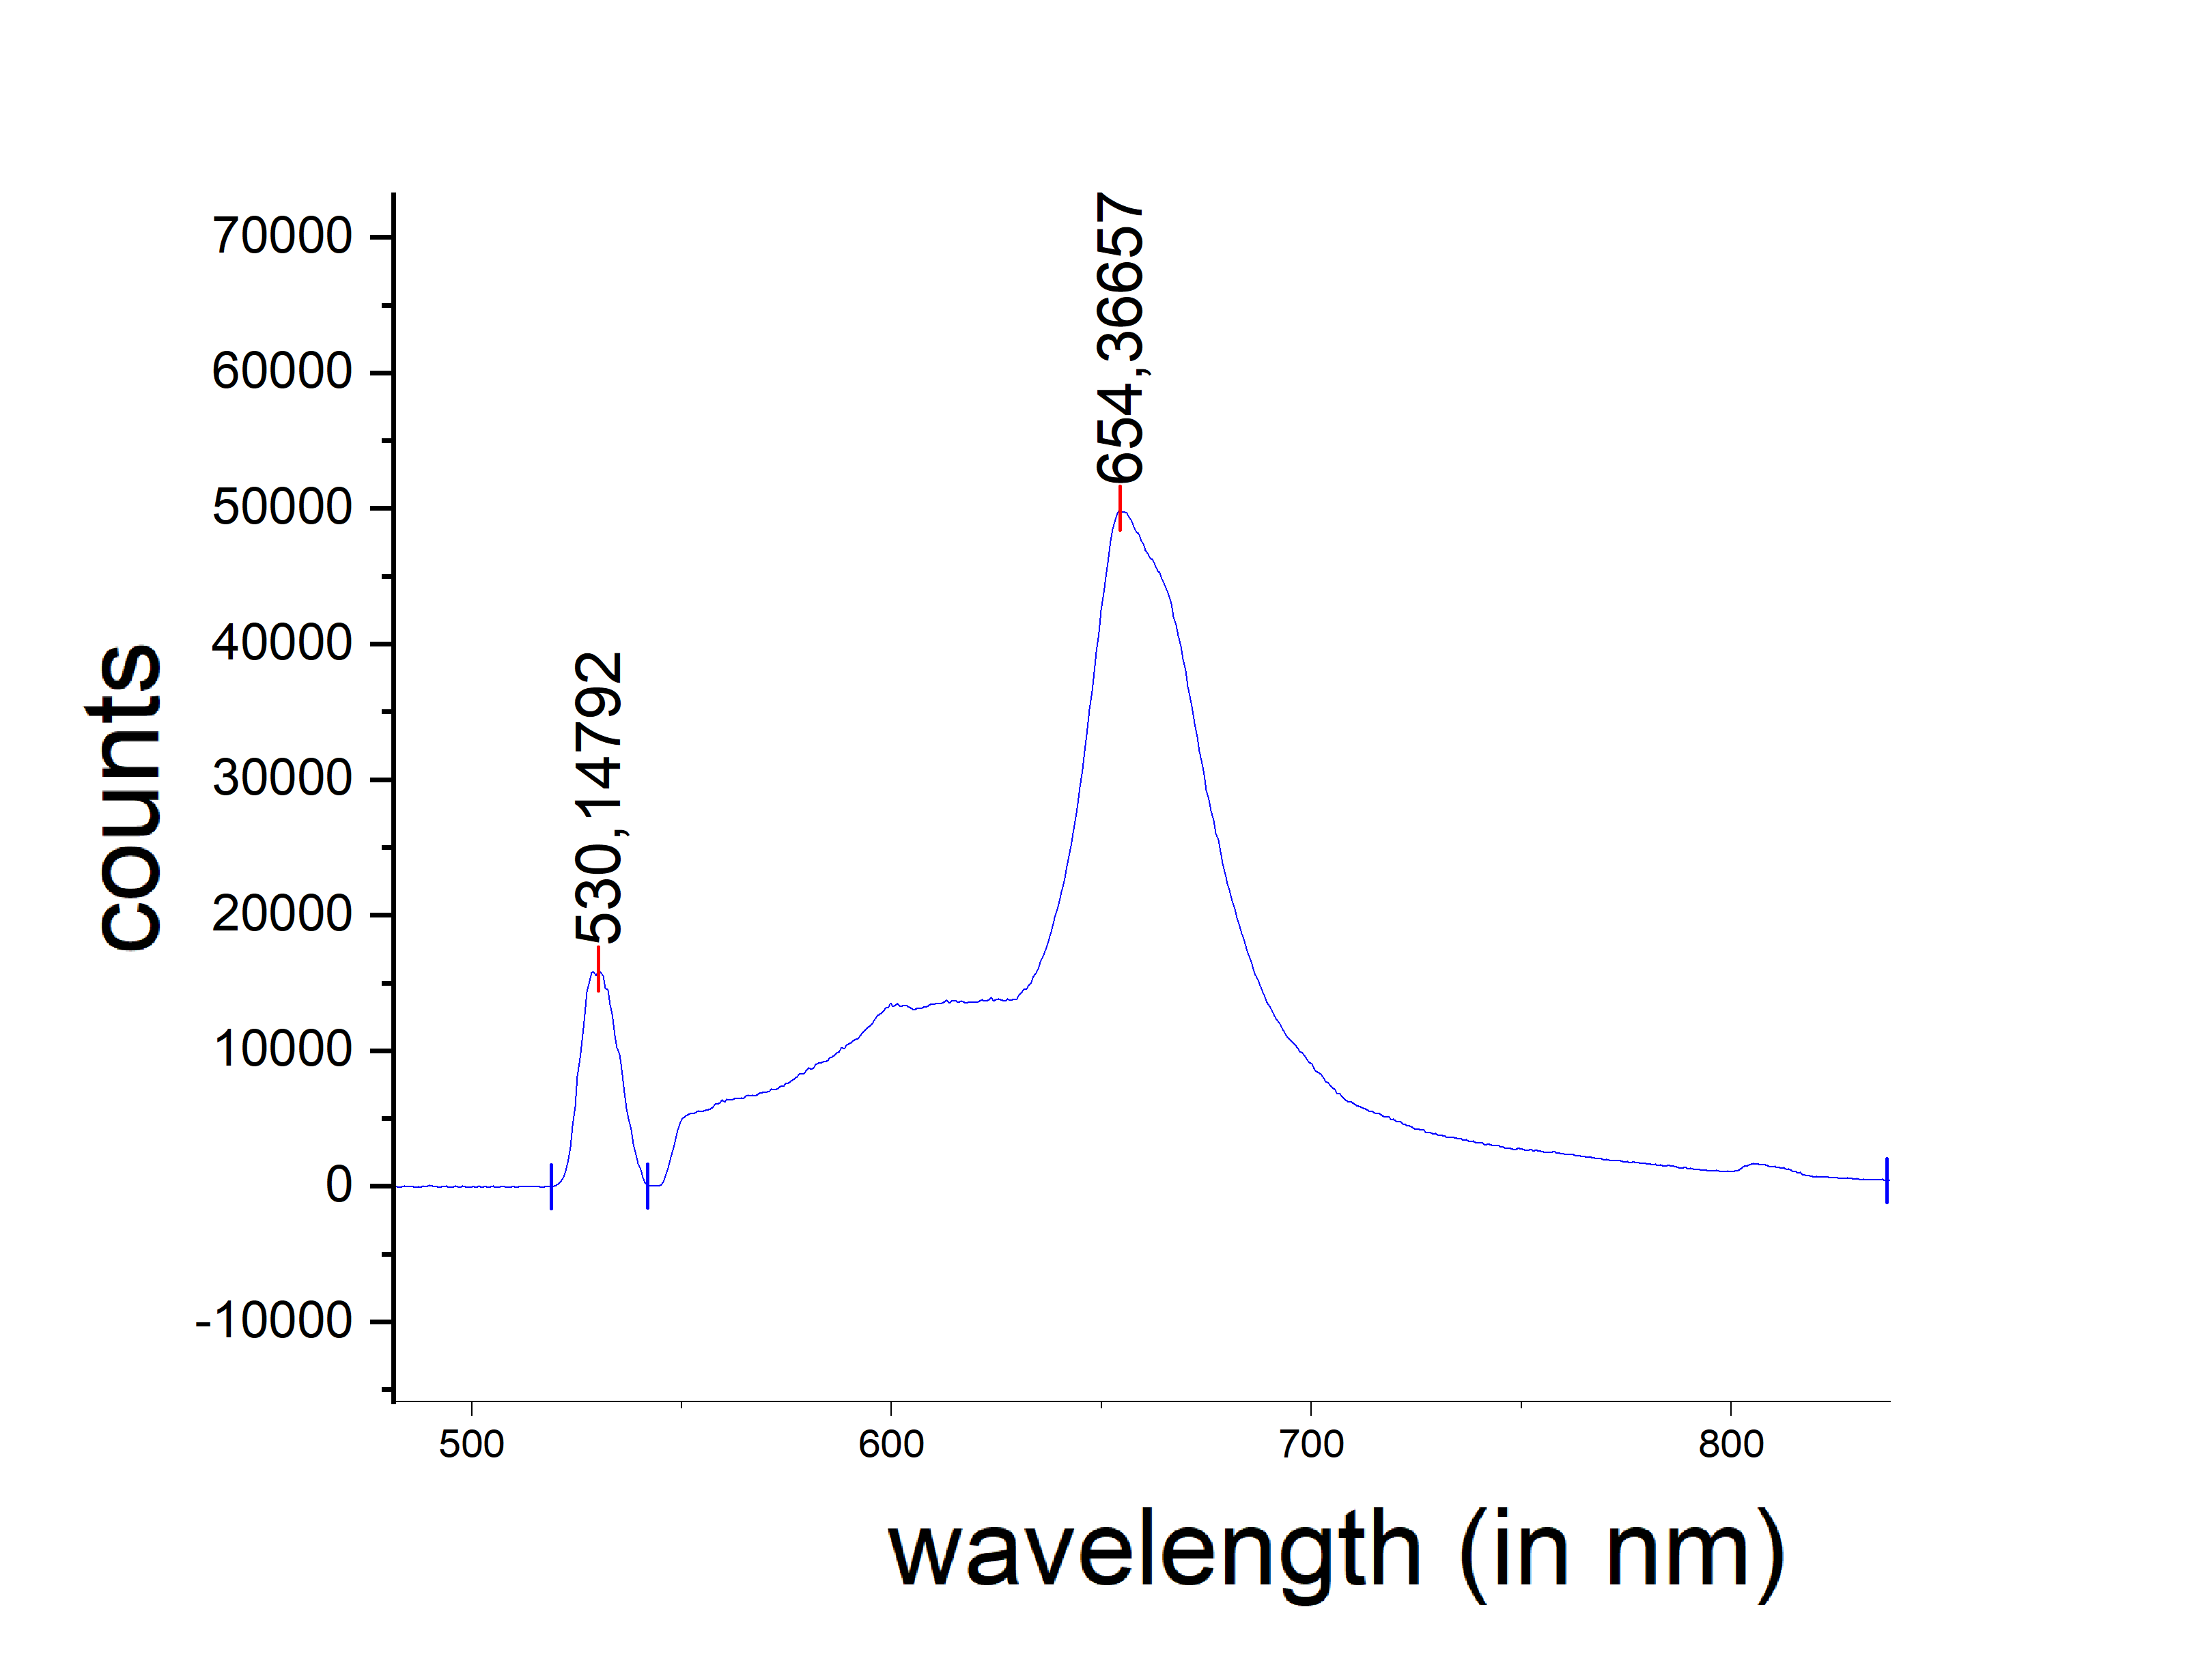
\includegraphics[width=\textwidth]{img/output_t1/spekt_m2}
        \caption{mat.2}
	      \label{fig_mono_spec3_1dspec}
    \end{subfigure}
    \caption{Measured Spectra for the two different materials. xc refers to the position of the peak and w is the FWHM.}
	\label{fig_mono_1dspectra} %mat2 -> 3
\end{figure}

From the spectra the peak positions and peak width are extracted, by performing a Gauss fit for each peak.
The peak width is given as the full width of the Gauss curve at half of its height (full width at half maximum, FWHM).
The peak position can be used to assign the materials to specific TMDCs according to their characteristic exciton transitions.
The measured peaks for material 1 are at \SI{746,5\pm 7,2}{nm} and \SI{744,1 \pm 7,2} for specimen 1 and 2, respectively, which corresponds well to WSe$_2$ monolayers, which are reported to emit at \SI{752}{nm}. \cite{Tonndorf2013}.

The measured peaks for material 2 lie at \SI{530,1 \pm 4,3}{nm} and \SI{654,4 \pm 6,8}.
The uncertainties are taken from the FWHM according to $\sigma = \mathrm{FWHM}/(2\sqrt{2 \ln 2})$.
The first peak can be assigned to the wavelength of the laser used (\SI{532}{nm}), meaning that the peak stems from leakage of the long pass filter.
The offset of \SI{2}{nm} is likely due to worse calibration of the spectrometer at the edges of the measurement range.
Using the Varshni equation and fit parameters as described and reported in \cite{xu19} at room temperature (\SI{295 \pm 5}{K}) monolayer MoS$_2$ emits at \SI{664 \pm 12}{nm}.
This allows the second peak to be assigned to monolayer MoS$_2$.
The shoulder of the peak at about \SI{600}{nm} may be due to the less efficient B exciton, making the larger peak the A exciton.
